\chapter{Related Work}
\label{cha:related-work}

Adrian et. al (2016) presents \emph{L0, L1, L2}, the state of the art
event trigger algorithms currently used by the KM3NeT data acquisition
pipeline. The L0 trigger applies a threshold to the analog signals in
the PMTs and poses as the first level of filtration before the data is
transferred to the on-shore facility. At the on-shore facility, the L1
filtration is applied by identifying coincidences of two or more L0
hits originating from different PMTs within the same DOM in a time
window of 10ns. The time window is deduced by studying the scattering
of light in deep sea. As a final filtration to reduce the occurrence
of random coincidences from background noise, the L2 filtration is
applied which is able to reduce the random coincidences by half by
taking into account the known spatial orientation of the PMTs. The
notion of identifying causally related hits was first proposed by
Bakker et al (2011). In their paper the authors proposed the
\emph{Match 3B Criterion} which observes the distance between two
hits. This distance is then compared to the distance that a photon is
known to travel in sea water.

%% alonso2020graph
%% - GNN for particle flow event reconstruction in neutrino oscillation
%% experiments -

Deep Learning has been an integral part of Particle Physics
experiments \cite{radovic2018machine, sadowski2015deep, de2019machine,
  psihas2020review, terwilliger2017vertex} including but not limited
to real time analysis and particle property prediction
\cite{radovic2018machine}. Study of exotic particles such as
\emph{Higgs boson}, \emph{anti matter}, \emph{dark matter} and
\emph{quarks} is a highly sought after topic in this field. However,
exotic particles are extremely difficult to detect due to the presence
of negligible charge and mass. Additionally, once created, they are
highly unstable and quickly decay into more stable forms
\cite{sadowski2015deep}. Thus to study exotic particles, the
conditions prevalent during the \emph{Big Bang} are recreated in large
collision experiments such as the ones conducted in the \emph{Large
Hadron Collidor (LHC)}. Since the particles cannot be detected
directly, the collision chambers are fitted with a plethora of sensors
and detectors to collect the direction and momentum of each particle
in order to recreate the collision event \cite{sadowski2015deep}.
These experiments produce data in the order of magnitude of
\emph{Petabytes} majority of which is just noise. To give an example,
the LHC produces $10^{11}$ particles out of which only 300 may be a
Higgs boson \cite{sadowski2015deep}. Due to the availability of an
abundance of data and the ``data hungry'' nature of Neural Networks,
the adoption of \emph{Deep Learning (DL)} for solving large scale
problems in the field was only a natural step. Based on a study on the
use of Machine Learning in neutrino experiments conducted by Psihas et
al (2020), DL models such as MLPs and CNNs have been applied to a
variety of physics problems such as design, hardware triggers, energy
estimation, reconstruction and signal selection. Many ML models have
replaced their statistical predecessors since they provide better
results.

A notable application of DL was in the discovery of the \emph{Higgs
boson} particle from data generated by the LHC collision experiments
\cite{radovic2018machine}. The same paper makes use of
\emph{Convolusional Neural Networks (CNNs)} and \emph{Recurrent Neural
Networks (RNNs)} for identification of \emph{beauty-quark} particles
where the data was represented in a graph structure. Sadowski et al.
(2015) employed ML techniques to reduce the dimensionality of the raw
dataset and compared the performance of shallow and deep MLPs for
identification of Higgs boson particles. CNNs have been widely adopted
for event recreation tasks since the data is often represented in the
form of images. Terwilliger et al. (2017) present such an application
where CNNs were used for \emph{neutrino vertex reconstruction} which
is a technique used to identify the origin of neutrino event using
detector data represented as images.

%% TODO needs more work, a bit "fika" <- Shru
All particle physics problem share the problem of having a high noise
to signal ratio in their datasets and ML techniques have been used to
tackle this problem \cite{mulmule2020machine, li2018deep,
  choma2018graph, neff2012signal}. In the deep sea environment in
which the \emph{ANTARES} neutrino telescope resides, \emph{Random
Forest} and \emph{Boosting Trees} were used for signal classification
\cite{neff2012signal}. Li et al. (2018) created a liquid neutrino
detector toy model to replicate the conditions posed by the
\emph{JUNO} detector. The image data generated by the toy model was
used to train CNNs to perform signal-noise discrimination and the
model was able to outperform the existing solutions. Choma et al.
(2018) used \emph{Graph Neural Networks} to perform signal-noise
detection using data collected by the \emph{IceCube} detector and the
model was able to outperform physics based methods and CNNs. Above the
ground, Mulmule et al. (2020) proposed the use of \emph{MLPBNN} a
Bayesian extension of MLPs for signal-background detection of
anti-neutrinos in the \emph{ISMRAN} experiment. The performance of the
model is better compared to the previously used statistical models
based on likelihood estimates.

Under the umbrella of the KM3NeT research initiative, three scientific
works of relevance to this project exist. The earliest being the paper
by De Sio et al. (2019) which presents the application of CNNs for
tasks such as event-type and particle identification, energy/direction
estimation, source identification, signal/background discrimination
and data analysis. The ML models provided better results compared to
the reconstruction models. Moreover, they alleviate the requirement
for reconstruction models altogether and extract relevant features
from the raw data directly. Post et al (2019) applied CNNs
\cite{krizhevsky2012imagenet} along with \emph{Long Short Term Memory
(LSTM)} \cite{sainath2015convolutional} for event triggering using
simulated KM3NeT data. The model performs a multi-class classification
amongst hits originating from noise, neutrinos and \emph{atmospheric
muons}. The model has promising results as it is able to attain an
accuracy of 80\%. Karas et al. (2019) builds upon the idea of causally
related hits by Bakker el al (2011) and presents a data processing
pipeline to filter timeslices containing hits from neutrino events
from those containing only noise. The pipeline is able to achieve this
filtration by processing the data in 3 steps, illustrated in Figure
\ref{fig:karas-pipeline} and described in more detail below. Figure
\ref{fig:karas-pipeline-data} provides a visual representation of the
various shapes and arrangements of the data as it passes through the
pipeline.

\begin{figure}[h]
  \centering
  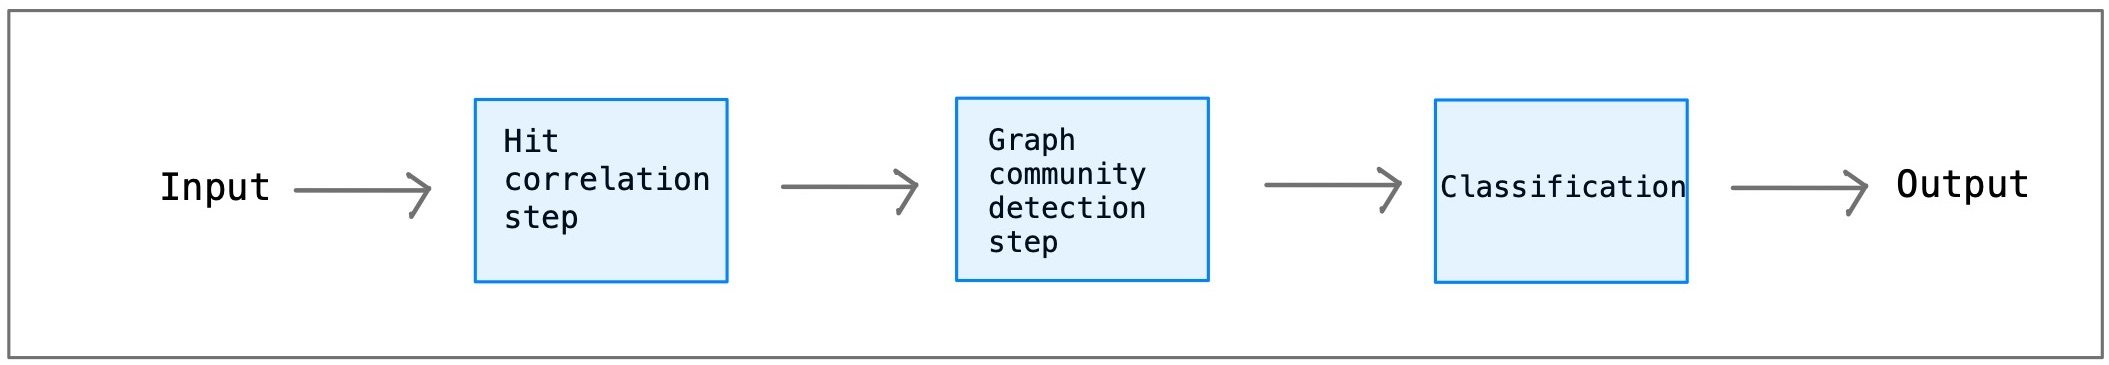
\includegraphics[width=\textwidth]{karas-pipeline.jpg}
  \caption{Overview of Karas Pipeline}
  \label{fig:karas-pipeline}
\end{figure}

\begin{figure}[h]
  \centering
  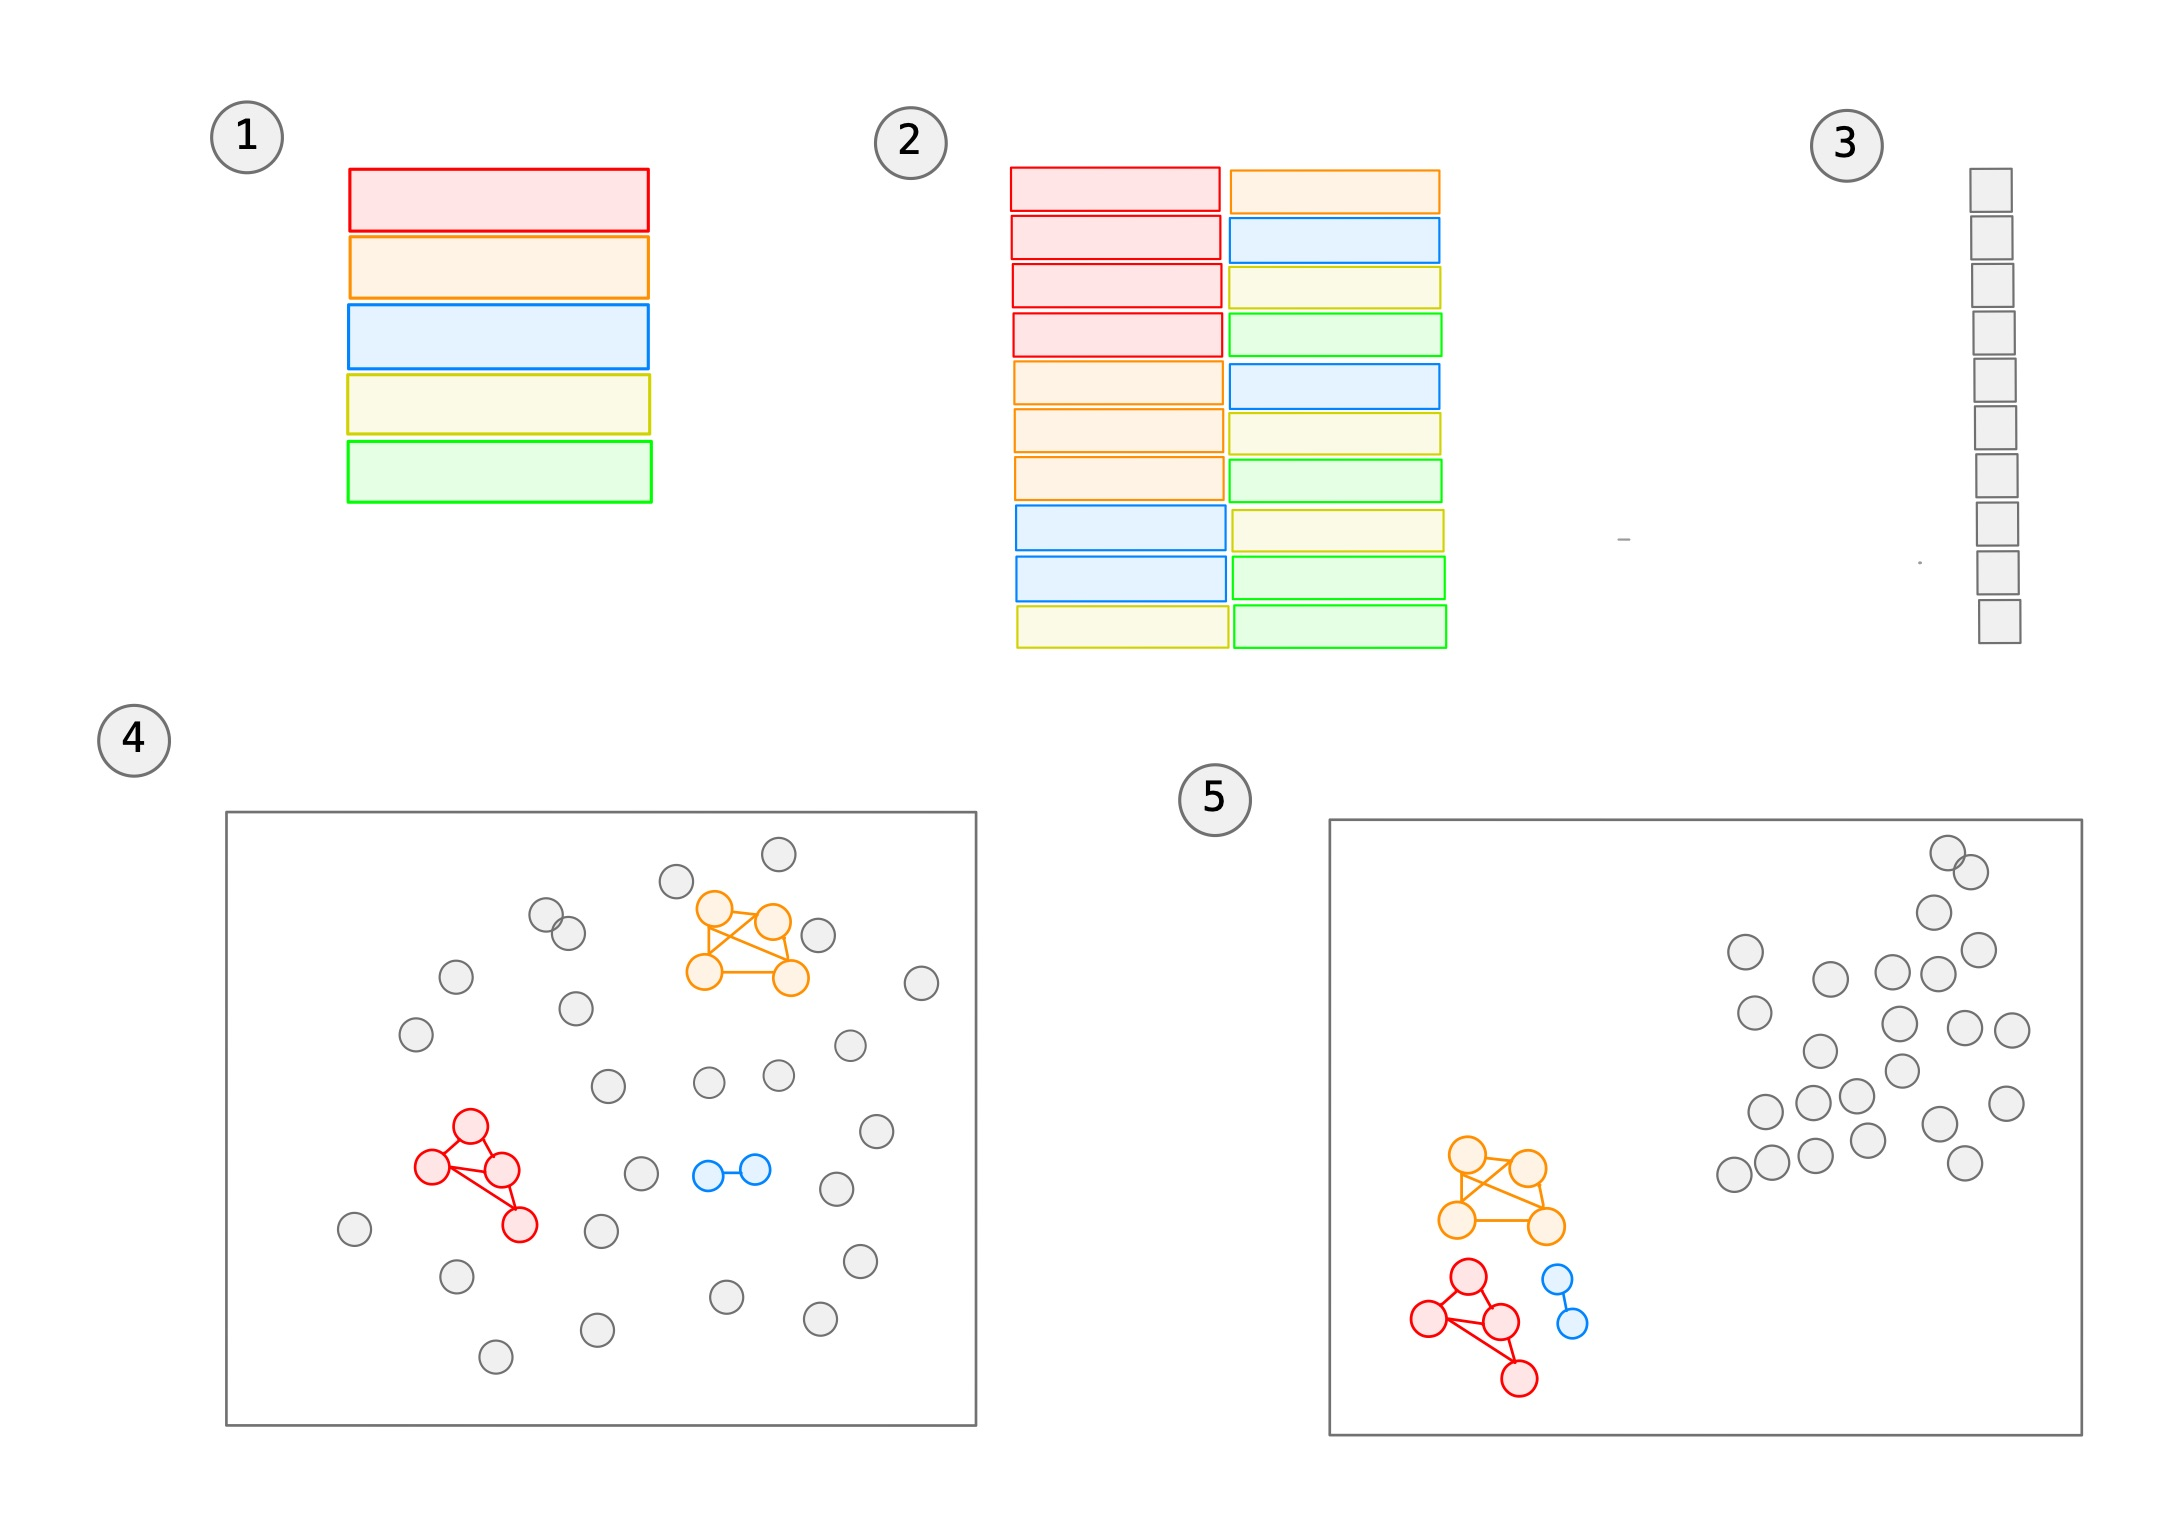
\includegraphics[width=\textwidth]{karas-pipeline-data.jpg}
  \caption{\textbf{(1)}. The dataset of the project where each row
    represents a hit consisting of the $(x, y, z, t) vector$. Here an
    example set containing 5 hits is shown. \textbf{(2)}. The input to
    the Hit Correlation Step is all unique pairs of hits.
    \textbf{(3)}. The output of the Correlation Step is a vector
    containing the probability that the pairs of hits are related to
    each other. \textbf{(4)}. (1) and (3) are used to construct a
    graph representation of the dataset where event (red, orange and
    blue) and noise (grey) hits are represented as nodes and are
    connected by an undirected edge carrying as weight the probability
    of being related (for simplicity, the edges are not shown).
    \textbf{(5)}. The graph from (4) acts as the input to the Graph
    Community Detection step, the output of which is another graph
    where event and noise nodes are grouped together and thus are
    linearly separable from each other.}
  \label{fig:karas-pipeline-data}
\end{figure}

The first step of The GPU pipeline is the Hit Correlation step which
proposes \emph{The Pattern Matrix Criterion (PMC)} to identify hits
which may have originated from the same neutrino event, referred to as
\emph{causally related} hits. From domain knowledge, it is known that
related hits occur close to each other both in space and time.
Specifically, the space and time difference of related hits is found
to be 100m and 300ns respectively \cite{adrian2016letter}. The PMC
operates by creating a correlation criterion based on the probability
that the aforementioned space and time difference occurs between two
related hits. Pairs of hits (from both events and noise) are passed to
the PMC as input, the output being an adjacency matrix where related
hits are assigned a high score whilst unrelated hits are assigned a
lower score. The algorithm is evaluated with a dataset containing 130
event hits and 5000 noise hits and results in the range of 0.3 - 0.375
is reported for the recall, precision and F1 metrics and an accuracy
of 80\% is achieved. Due to the stocastic nature of hits, unrelated
hits such as noise-event or noise-noise pairs may occur within this
predefined range thus being falsely identified as related. This is
rectified in the next step of the pipeline.

The second step of the Karas pipeline is the Graph Community Detection
(GCD) step. The main dataset is represented as a graph where hits are
represented as nodes. All nodes are connected with each other and
carry as weight the probability of being related using the output of
the PMC. The \emph{Constant Potts Model (CPM)} \cite{traag2011narrow}
is used to group the nodes into separate communities (or clusters) of
related and unrelated hits. The model is tested using a dataset
consisting of 130 event hits and 5000 noise hits and performs
exceptionally well as it is able to group most event hits into a
single community and the noise in another.

Since the GCD step directly operates on the data derived using the Hit
Correlation step, communities may still contain noise nodes. Thus the
third and final step of the pipeline classifies given communities as
\emph{event} or \emph{noise} communities based on the exclusive
presence of event nodes. This can be done by observing two properties
of the graph namely the size of the communities and the density of
edges within the communities. Communities consisting exclusively of
event nodes are of small sizes and have high edge density whilst
communities consisting a mix of event and noise nodes or only noise
nodes will be relatively larger and have lesser edge density. The two
parameters which aid in the classification are the Probability
Threshold (PT) of the PMC and the CPM resolution parameter ($\gamma$)
of the GCD step. The PT and $\gamma$ are grid searched to determine
their optimal thresholds, all hits above the specified thresholds are
classified as event communities and the rest as noise communities.

Although The Karas Pipeline is able to identify timeslices with
neutrino event hits more accurately compared to its predecessors
\cite{karas2019data}, the pipeline still has certain limitations which
hinders its performance. The space and time difference based on which
the PMC determines if two hits are causally related to one another is
static. This may result in related hits which do not meet these
thresholds to be incorrectly given a low score. Alternatively, due to
the stocastic nature of hits, event-noise and noise-noise pairs which
fall within the thresholds may also occur and these will be
incorrectly given a high score. The communities created by CPM is
influenced by the edge weights provided by the PMC thus any
limitations of the PMC cascades down into the later steps of the
pipeline. Furthermore, the classification step also operates on static
values of the PT and $\gamma$ and thus is unable to identify
communities of size smaller than 20 hits.

Instead of deriving the correlation thresholds manually, a better
approach may be to use NNs to learn the optimal thresholds. This idea
is further explored in Chapter \ref{cha:mlp} where a MLP is used to
classify related and unrelated hits. Recently, the field of Geometric
Deep Learning has gained popularity with some exciting developments of
models which are designed to operate upon graph structures. Once such
development is the Graph Convolusional Neural (GCN) Network proposed
by Kipf et al (2016). The limitations of the GCD and classification
steps may be alleviated by using a GCN to classify event and noise
nodes and is explored in Chapter \ref{cha:gcn}.
